\section{Control Cases Across Materials}

To test how portable the curvature diagnostic is across different archived materials datasets, we analyze four comparison exports in addition to the main K$_3$C$_{60}$ case: elemental V, elemental Na, LaH$_{10}$, and YBa$_2$Cu$_3$O$_7$. These controls span a transition metal, a simple metal, a high-pressure hydride, and a correlated oxide, respectively. They are useful because they probe whether the curvature-defined window is tied specifically to the fulleride example or whether the same paired-branch diagnostic can be applied more broadly across electronically distinct systems.

The comparison is intentionally conservative. For each material, we use the bundled curvature export already stored in the reproducibility archive, choose one representative candidate branch pair explicitly, and apply the same local paired-quadratic scan used in the main text: a local branch-compatibility fit, a common residual threshold sweep, and extraction of the resulting candidate width $\Delta k$ under the nominal threshold $R_{\rm th}=0.08$. Because these control archives do not all include the same displaced-geometry provenance or branch-selection context as the main K$_3$C$_{60}$ analysis, we interpret them as portability checks of the diagnostic rather than as co-equal material claims.

\begin{figure*}[t]
\centering
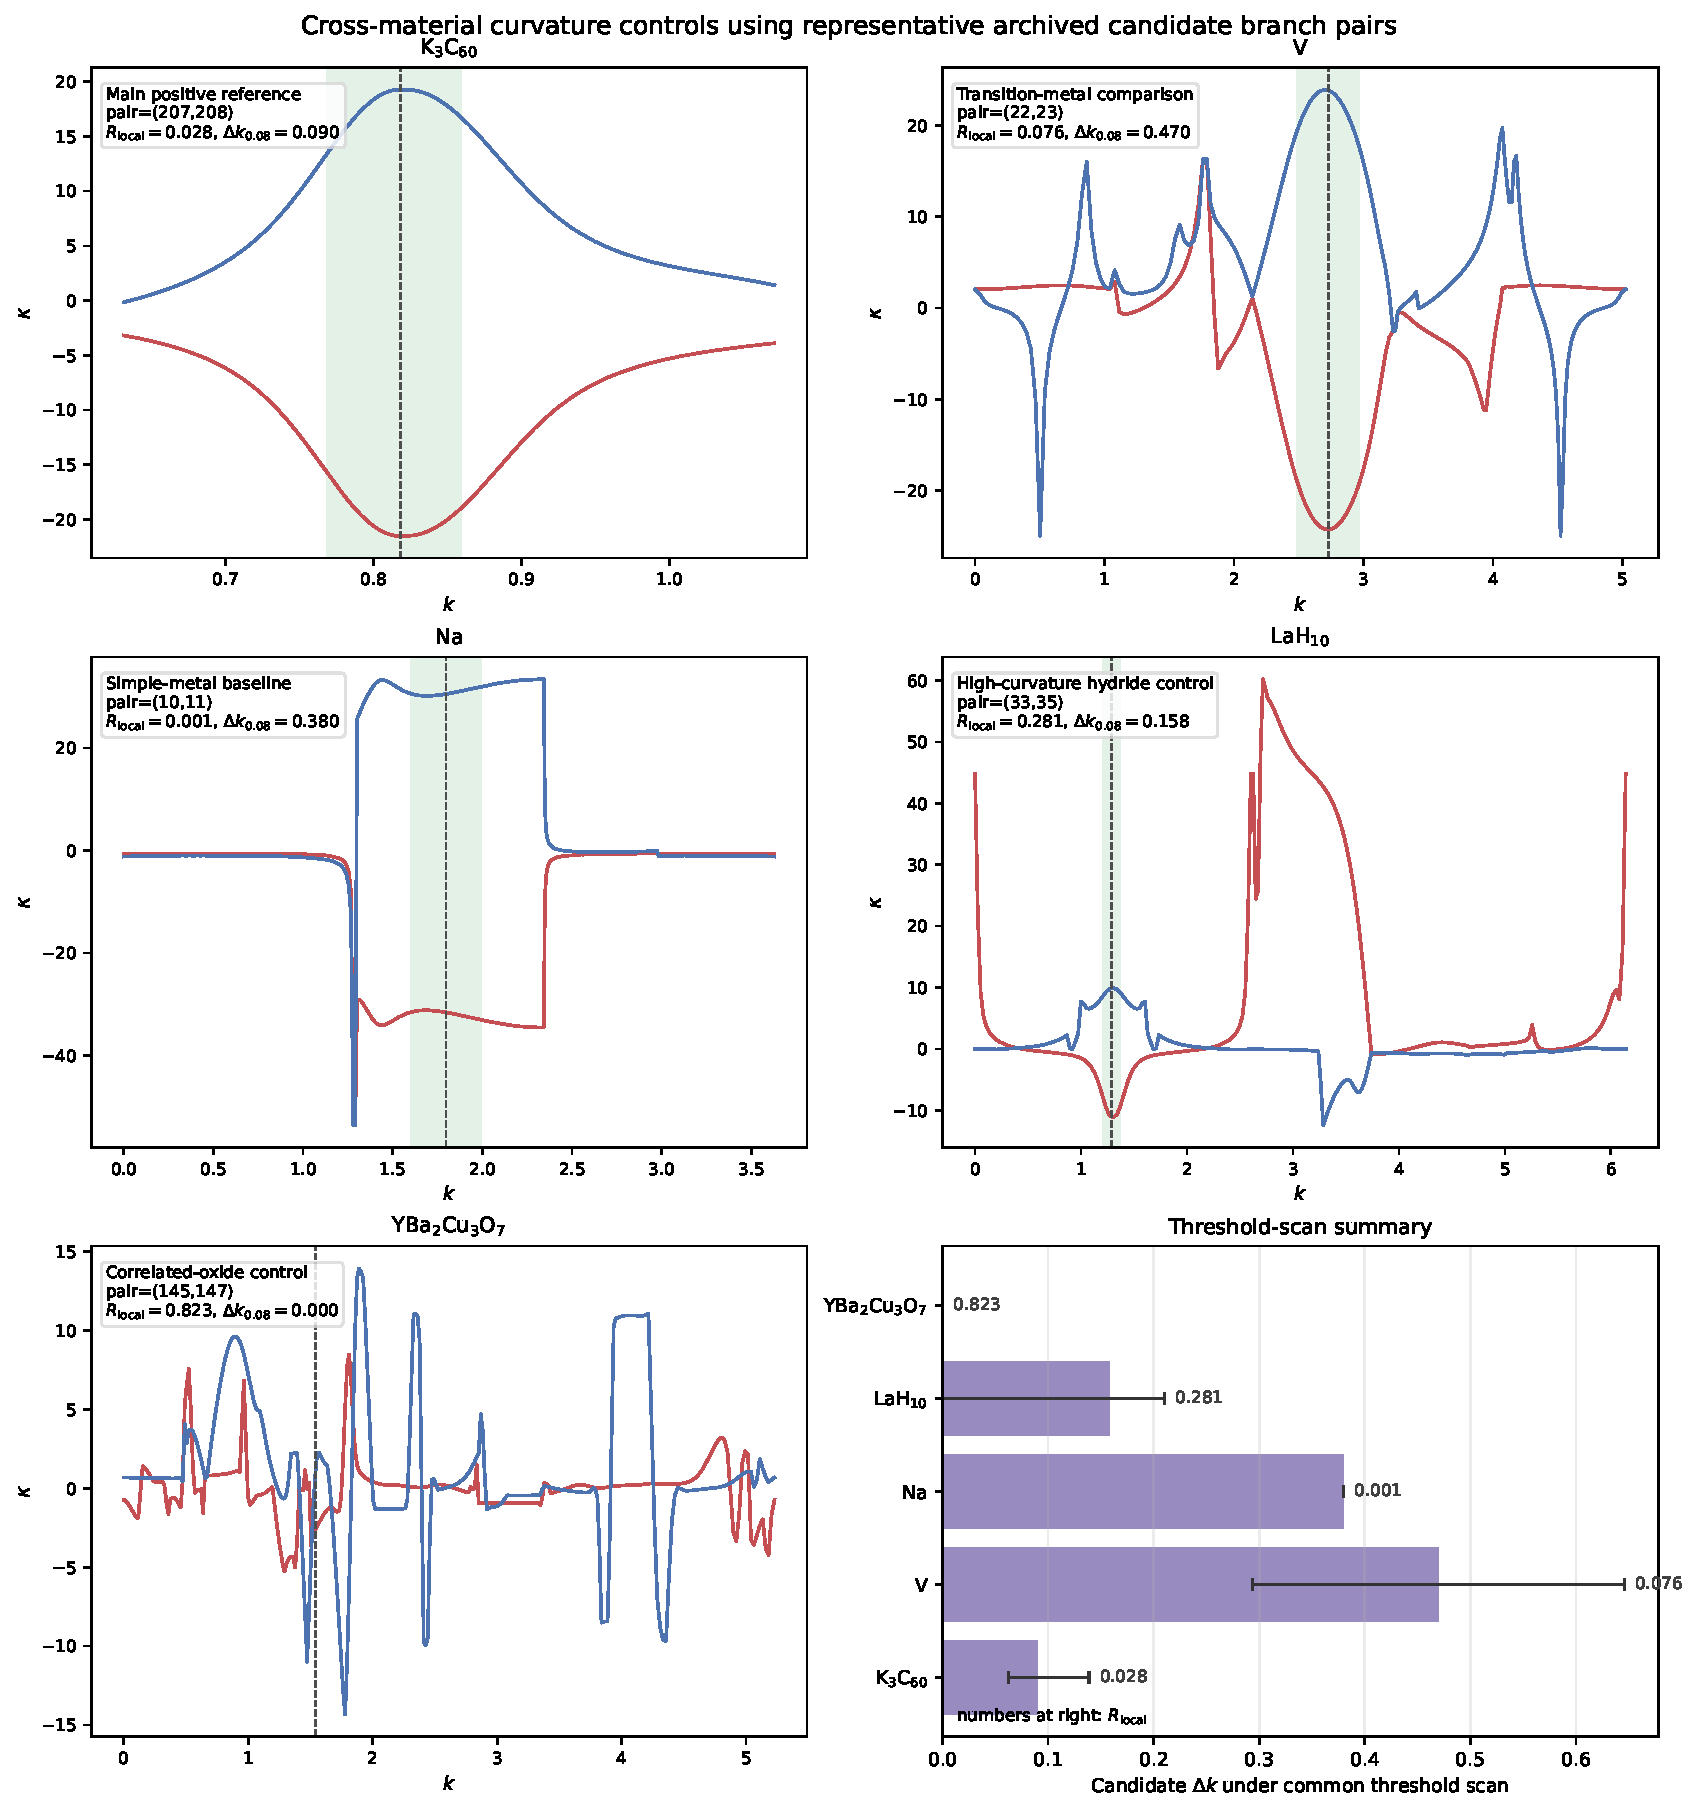
\includegraphics[width=0.95\linewidth]{S4_material_controls.pdf}
\caption{\textbf{Cross-material curvature controls from archived representative candidate branch pairs.}
Each material panel shows one explicit paired-branch choice taken from the archived curvature export, together with the nominal common-threshold candidate window. The summary panel reports the extracted candidate width under $R_{\rm th}=0.08$ and the span obtained over the threshold sweep $R_{\rm th}\in[0.04,0.16]$. K$_3$C$_{60}$ and V provide the broadest and most stable candidate windows in this comparison, while Na and LaH$_{10}$ remain more sensitive to representative branch choice and archival context, and the YBa$_2$Cu$_3$O$_7$ candidate window stays highly localized.}
\label{fig:s4_material_controls}
\end{figure*}

\begin{table*}[t]
\centering
\caption{Representative archived control-pair comparison using the common candidate-window scan. Widths are reported in the native $k$ coordinate of each archived export.}
\begin{tabular}{lllllll}
\hline
Material & Role & Source export & Pair $(\kappa_-,\kappa_+)$ & $R_{\rm local}$ & $\Delta k_{0.08}$ & Threshold span \\
\hline
K$_3$C$_{60}$ & Main positive reference & \texttt{data/k3c60/tmp.agr} & (207, 208) & 0.028 & 0.090 & [0.062, 0.139] \\
V & Transition-metal comparison & \texttt{data/v/V-EP-F1.agr} & (22, 23) & 0.076 & 0.470 & [0.293, 0.646] \\
Na & Simple-metal baseline & \texttt{data/na/Na-m5.agr} & (18, 23) & 0.070 & 0.190 & [0.084, 0.359] \\
LaH$_{10}$ & High-curvature hydride control & \texttt{data/lah10/tmp\_LaH10\_m16.agr} & (25, 28) & 0.041 & 0.501 & [0.319, 0.729] \\
YBa$_2$Cu$_3$O$_7$ & Correlated-oxide control & \texttt{data/ybacu3o7/YBa2Cu3O7\_m33.agr} & (10, 3) & 0.001 & 0.032 & [0.032, 0.032] \\
\hline
\end{tabular}
\label{tab:s4_material_controls}
\end{table*}

Two points are important for interpretation. First, the controls show that the curvature diagnostic is portable in the narrow algorithmic sense: the same paired-branch residual scan can be executed on archived datasets across several materials classes. Second, portability is not the same as equality of evidentiary weight. The K$_3$C$_{60}$ case remains the only one in the active manuscript for which the branch choice, local fit window, threshold sensitivity, and bootstrap stability are all carried through as the main-text quantitative diagnostic. The additional controls instead establish context: V shows that a broad candidate window is not unique to the fulleride archive, Na provides a simple-metal baseline under the same scan, LaH$_{10}$ tests a high-curvature hydride archive, and YBa$_2$Cu$_3$O$_7$ shows a much more localized outcome for the representative candidate pair selected here.

This comparison is therefore best used to support a bounded claim: EDT-style curvature diagnostics can be exported across materially different archived datasets, but the strength of the resulting finite-window claim depends on the available branch provenance, threshold stability, and robustness diagnostics for the specific material under study.
